

\chapter{Metodologia}

Neste capítulo são descritas as etapas de desenvolvimento do projeto que já foram implementadas, tendo em vista a proposta apresentada para construção de um produto de tecnologia assistiva para ensino de tipografia a deificientes visuais, mais especificamente, no caso deste trabalho, o sistema de classificação de tipografias.

O processo completo de desenvolvimento do sistema se deu em três etapas principais listadas a seguir:

\begin{enumerate}
\item Pesquisa bibliográfica e estudo dos conceitos basilares
\item Composição do banco de dados
\item Implementação do algoritmo para classificação das imagens
\end{enumerate}
%\ldots - reticencias

A primeira etapa deste trabalho foi caracterizada por pesquisa bibliográfica e estudos mais aprofundados em tipografia, princípios de processamento de imagens e aprendizado de máquina, além de debates para a idealização do produto final de tecnologia assistiva oferecido ao deficiente visual. Os resultados dessa etapa foram descritos no capítulo 2, como fundamentação teórica, e no capítulo 1, como apresentação da proposta de projeto. Porém, tópicos em relação ao projeto final do produto encontram-se na seção destinada a trabalhos futuros.

A segunda e a terceira etapas, por sua vez, foram desenvolvidas e aprimoradas simultaneamente. O processo de desenvolvimento adotado nessas etapas é explicitado abaixo.

\section{Composição do Banco de Imagens}

Como já descrito, foram escolhidas nove tipografias para o projeto e, para cada uma delas, construído um conjunto de imagens. Para melhor organização, o banco foi montado tipografia a tipografia. As imagens que compõem o banco de dados em sua versão final são caracteres separados de cada tipografia, amostras podem ser vistas na Figura \ref{fig:nimage}.


A principal fonte de obtenção das imagens originais foi o \textit{Fonts in Use}, um website que disponibiliza fotografias de projetos envolvendo design gráfico já classificadas por tipografia \citeC{fontsinuse2017}. Além deste, foram utilizados sites de busca convencionais, na opção de imagens. Ainda, para os casos em que poucas imagens foram encontradas, a saber as tipografias \textit{Franklin Gothic} e \textit{Adobe Jenson}, imagens complementares foram cedidas como cortesia.


\begin{figure}[H]
  \centering
  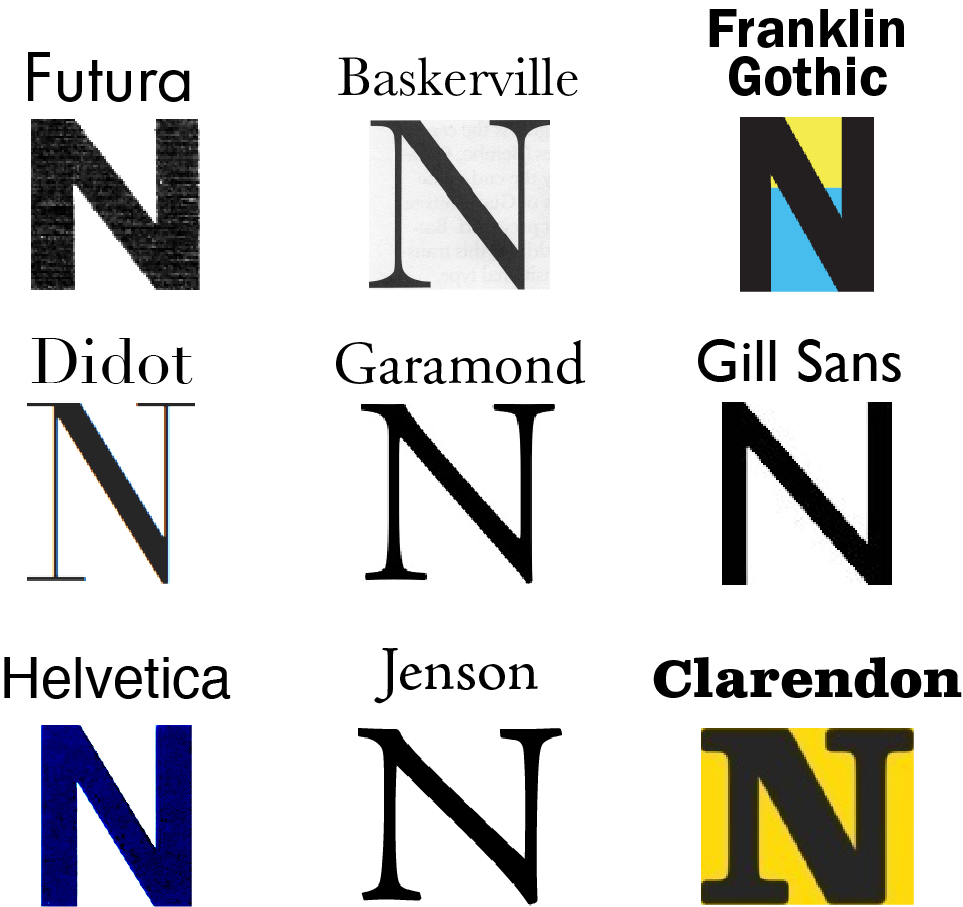
\includegraphics[width=0.5\linewidth]{figuras/nimage.pdf}
  \caption{Amostras do banco de imagens, especificando-se a tipografia - \textbf{Fonte:} Autora}
  \label{fig:nimage}
\end{figure}


É comum tipografias digitais apresentarem várias versões distintas entre si. Enquanto representações da versão física original dos tipos, as tipografias digitais possuem variações, pois diversas fundidoras de tipos propõem seu próprio modelo representativo para aquela tipografia. Um exemplo utilizando-se a tipografia Garamond é apresentado na Figura \ref{fig:comparacaoTipos}. Escolheu-se, para ilustração, a letra "a", sendo possível verificar as distinções presentes no formato de três partes específicas da letra: bojo, remate e terminal em gota. A versão adotada no projeto é a Adobe Garamond Pro. Logo, para a obtenção de cada imagem por meio de websites, foi necessária uma análise manual para verificar se tratava-se da tipografia correta, em sua versão empregada no projeto.


\begin{figure}[H]
  \centering
  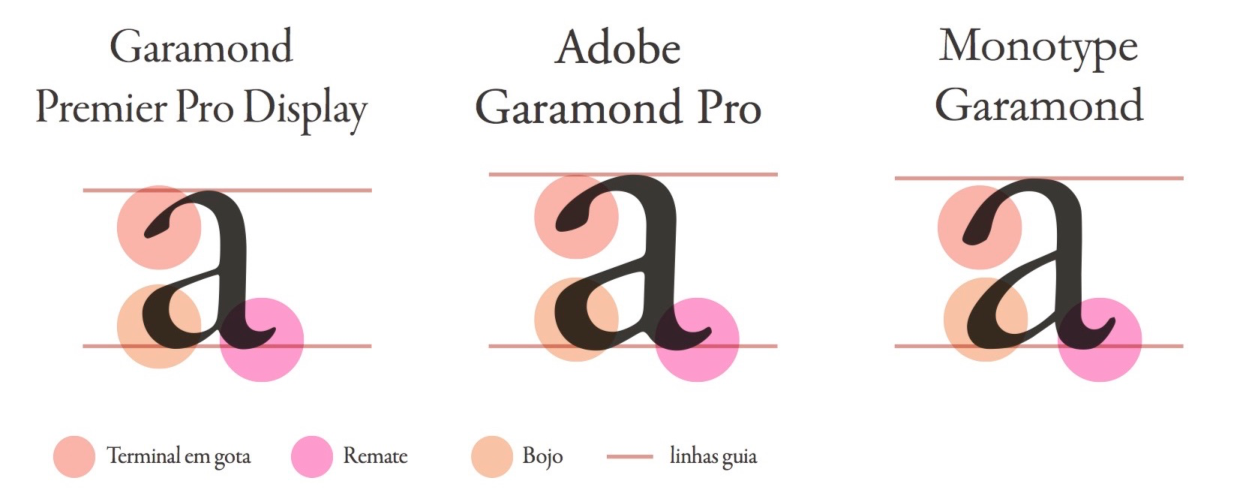
\includegraphics[width=0.8\linewidth]{figuras/comparacaoTipo.pdf}
  \caption{Comparação entre três versões da fonte Garamond, evidenciando as partes anatômicas distintas - \textbf{Fonte:} Autora}
  \label{fig:comparacaoTipos}
\end{figure}

Sendo assim, a adição de uma imagem de uma outra versão da tipografia poderia gerar um erro de classificação, já que algumas tipografias empregadas no projeto são bastante similares entre si, fato ilustrado na Figura \ref{fig:comparacaoJensonGaramond} que apresenta a similaridade entre duas tipografias presentes no projeto. Portanto, a análise foi realizada de forma minuciosa, utilizando conceitos da anatomia das letras, como o formato de suas serifas e o contraste entre as partes \citeC{rocha2004}. Ademais, as imagens originais obtidas muitas vezes continham variações que deveriam ser excluídas manualmente, como mais de uma tipografia em sua composição, ou então uma mistura entre os variados estilos dentro de uma família tipográfica: itálico, algumas variações de negrito e versalete, sendo um fator adicional na análise das imagens durante o processo.

\begin{figure}[H]
  \centering
  
\includegraphics[width=0.5\linewidth]{figuras/comparacaoJensonGaramond.pdf}
  \caption{Comparação entre as fontes \textit{Adobe Garamond Pro} e \textit{Adobe Jenson Pro}, atestando o alto índice de similaridade entre elas - \textbf{Fonte:} Autora}
  \label{fig:comparacaoJensonGaramond}
\end{figure}

Para o processo de separação das imagens em caracteres únicos, implementou-se um algoritmo em Python para automatização do processo de reconhecimento da localização dos caracteres na imagem e de formação de novas imagens individuais, algo similar a "recortes" {} da imagem original. A principal biblioteca utilizada nesse algoritmo foi a \textit{OpenCV} (\textit{Open Source Computer Vision Library}), uma biblioteca de visão computacional e aprendizado de máquina disponível em código livre (\textit{open source}). Ela foi escolhida por ser amplamente utilizada por especialistas da área e em empresas renomadas como Google, Microsoft, Intel e IBM \citeC{opencv2017}.

O algoritmo é composto de uma seção principal denominada \texttt{mainBancoDados} e módulos importados, que incluem os métodos (estruturas em Python análogas à funções) implementados para desempenhar operações específicas nas imagens. O leitor pode acompanhar a descrição do código por meio do fluxograma na Figura \ref{fig:flowMain} para melhor entendimento. Ao executar o algoritmo, deve-se escolher em qual parte do banco de dados, ou seja, em qual fonte deseja-se atuar. A seção principal dá acesso à execução de três operações: recorte das imagens originais, exclusão das imagens de dimensão insatisfatória e renomeação das imagens.

Ao responder positivamente à operação de recorte de imagens, chamam-se o método \texttt{imCrop} e o método de exclusão de imagens \texttt{imApaga}, importados de módulos implementados. Caso a resposta à essa operação seja negativa, passa-se para a seleção da operação de exclusão de imagens. Se a resposta for positiva, chama-se o método de exclusão de imagens, seguindo para a seleção da renomeação das imagens após a execução da operação ou caso a resposta tenha sido negativa. Por fim, frente à resposta positiva para renomeação das imagens, o método \texttt{changeName} é chamado, finalizando a execução do algoritmo, em caso negativo, a finalização ocorre imediatamente.


\begin{figure}[H]
  \centering
  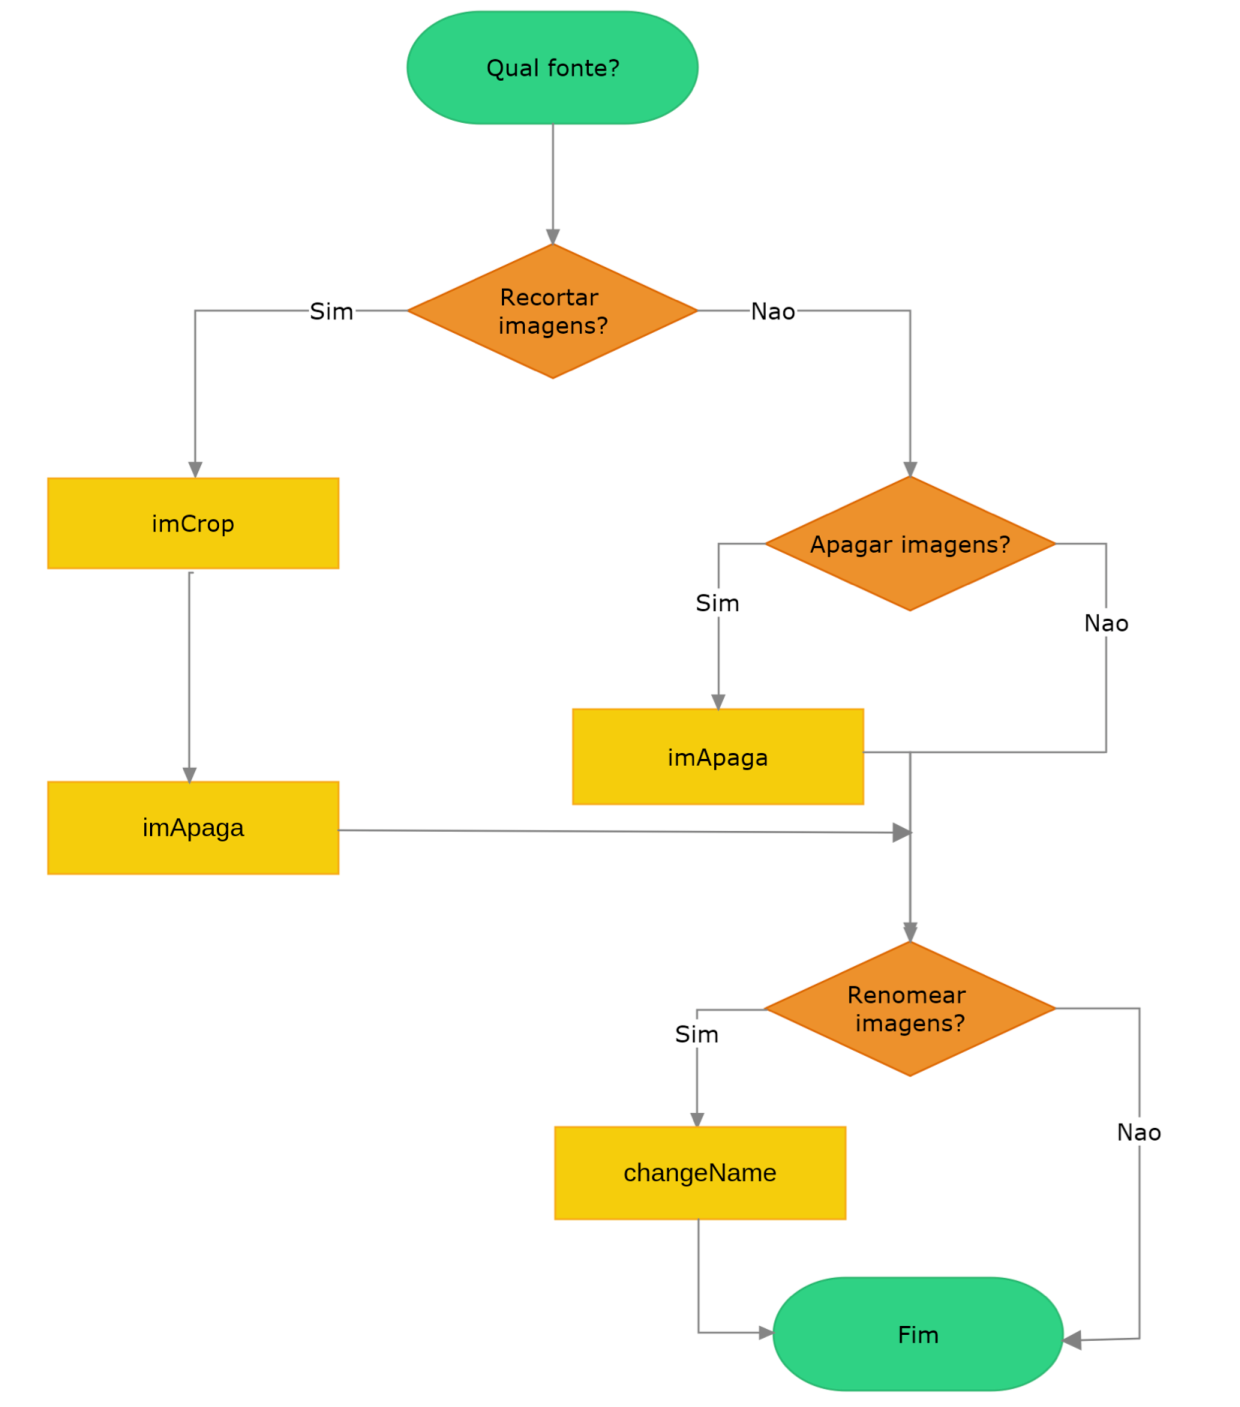
\includegraphics[width=0.9\linewidth]{figuras/mainbancodados.pdf}
  \caption{Fluxograma da seção principal do algoritmo para composição do banco de dados - \textbf{Fonte:} Autora}
  \label{fig:flowMain}
\end{figure}

Passa-se, então, para a descrição de cada um desses métodos separadamente. Em primeiro lugar, o método \texttt{imCrop} performa o recorte das imagens originais, criando imagens individuais de caracteres e seu fluxograma está apresentado na Figura \ref{fig:flowimCrop}. Quando chamado na seção principal, o método \texttt{imCrop} recebe como parâmetro de entrada o nome da fonte em que se deseja operar, já que o banco de imagens divide-se por tipografias, então, o diretório de operação passa a ser o banco de imagens da fonte escolhida. Todas as imagens contidas naquele diretório são convertidas para o formato \textit{PNG}, pois é um dos formatos aceitos pela biblioteca \textit{OpenCV}.


\begin{figure}[H]
  \centering
  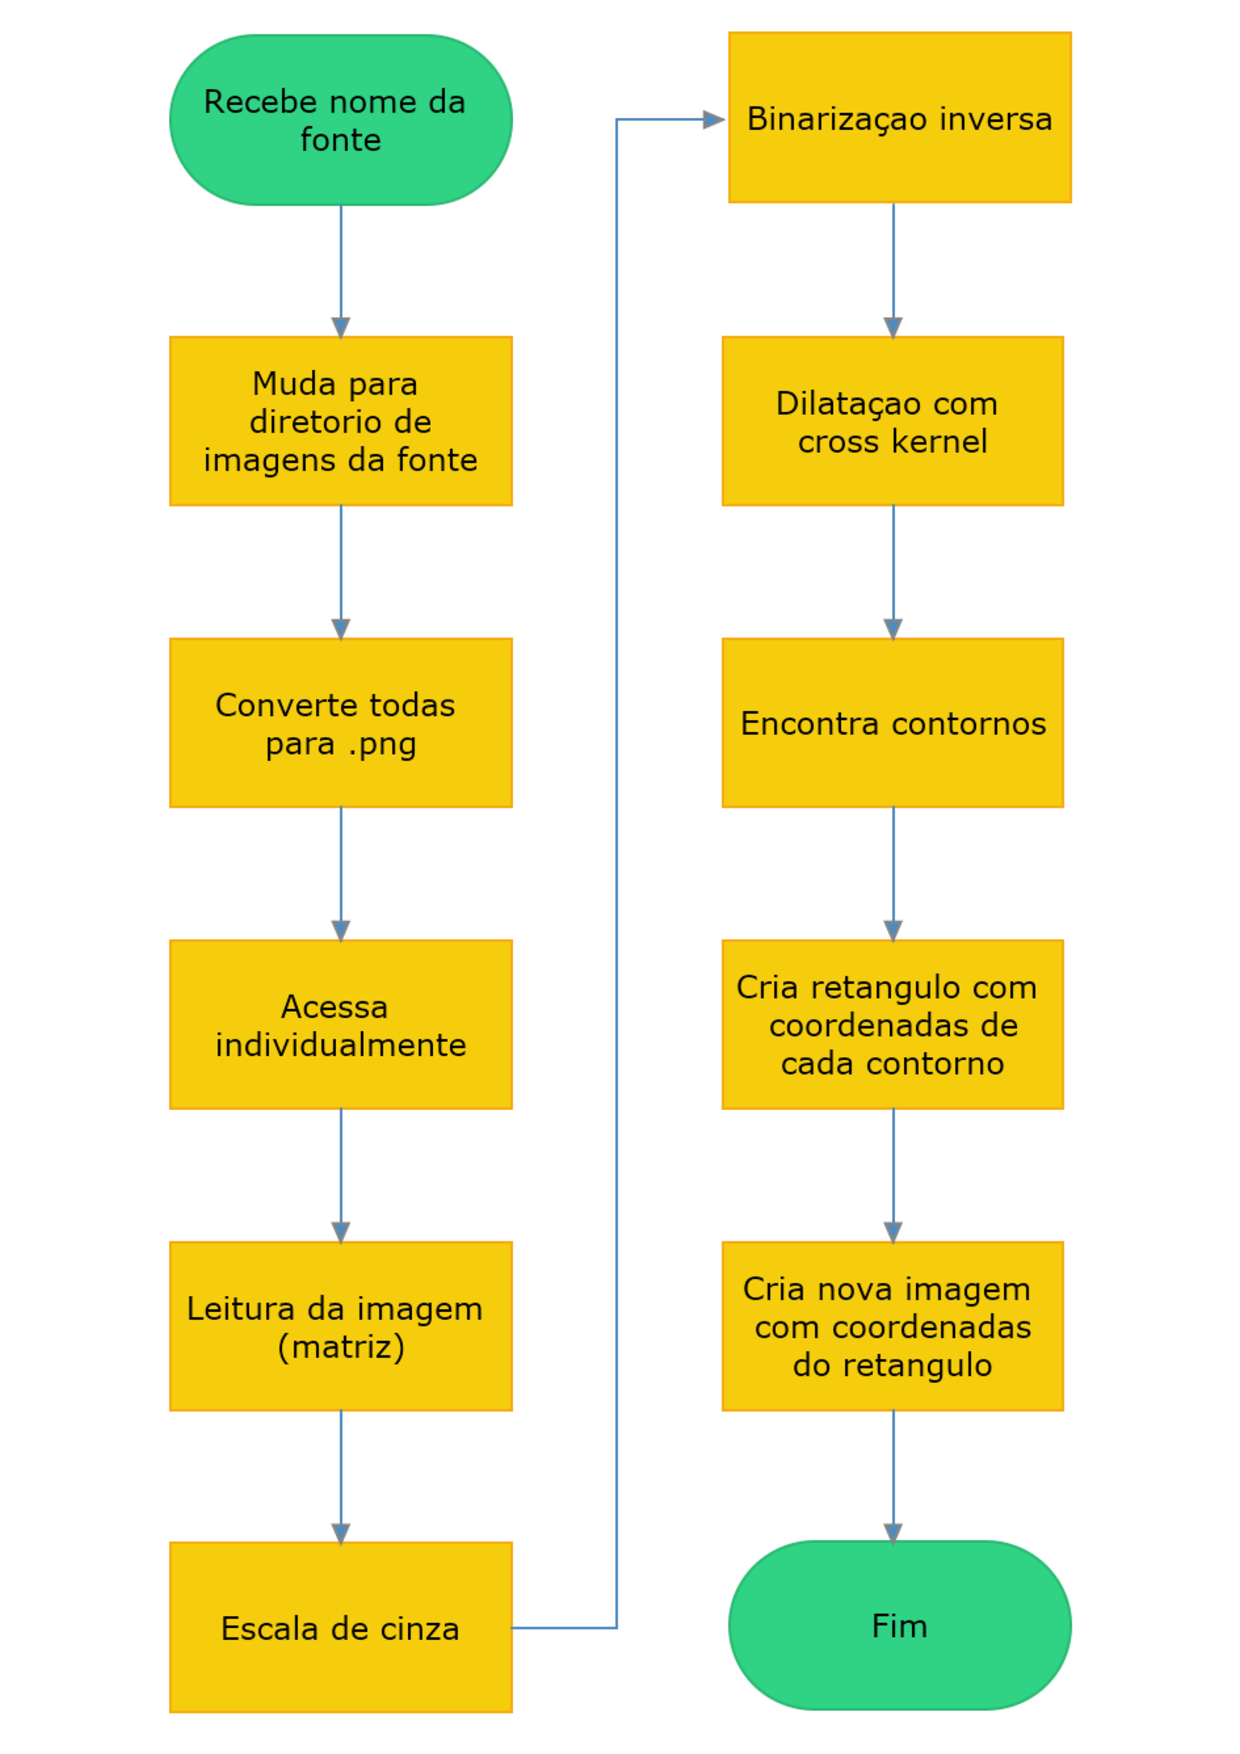
\includegraphics[width=0.7\linewidth]{figuras/imCrop.pdf}
  \caption{Fluxograma do método \texttt{imCrop} para recortar as imagens originais, criando imagens separadas de cada caractere  - \textbf{Fonte:} Autora}
  \label{fig:flowimCrop}
\end{figure}

As imagens são acessadas individualmente, e lidas uma por vez, ou seja, armazenados os valores de seus pixels em uma matriz. A imagem é alterada para escala de cinza, faz-se a sua binarização inversa utilizando um limiar de nível 88, ou seja, valores acima são assinalados como preto e valores abaixo, branco. O próximo passo é a dilatação usando um \textit{kernel} em cruz, com dimensão 3x3. Após isso, encontram-se os contornos de cada parte branca da imagem. São criados retângulos limitadores ao redor dessas partes utilizando as coordenadas dos contornos e novas imagens são criadas a partir desses retângulos. Todo o processo é exemplificado a partir de uma imagem da fonte Futura na Figura \ref{fig:imProcess}, para acompanhamento do leitor.

\begin{figure}[H]
  \centering
  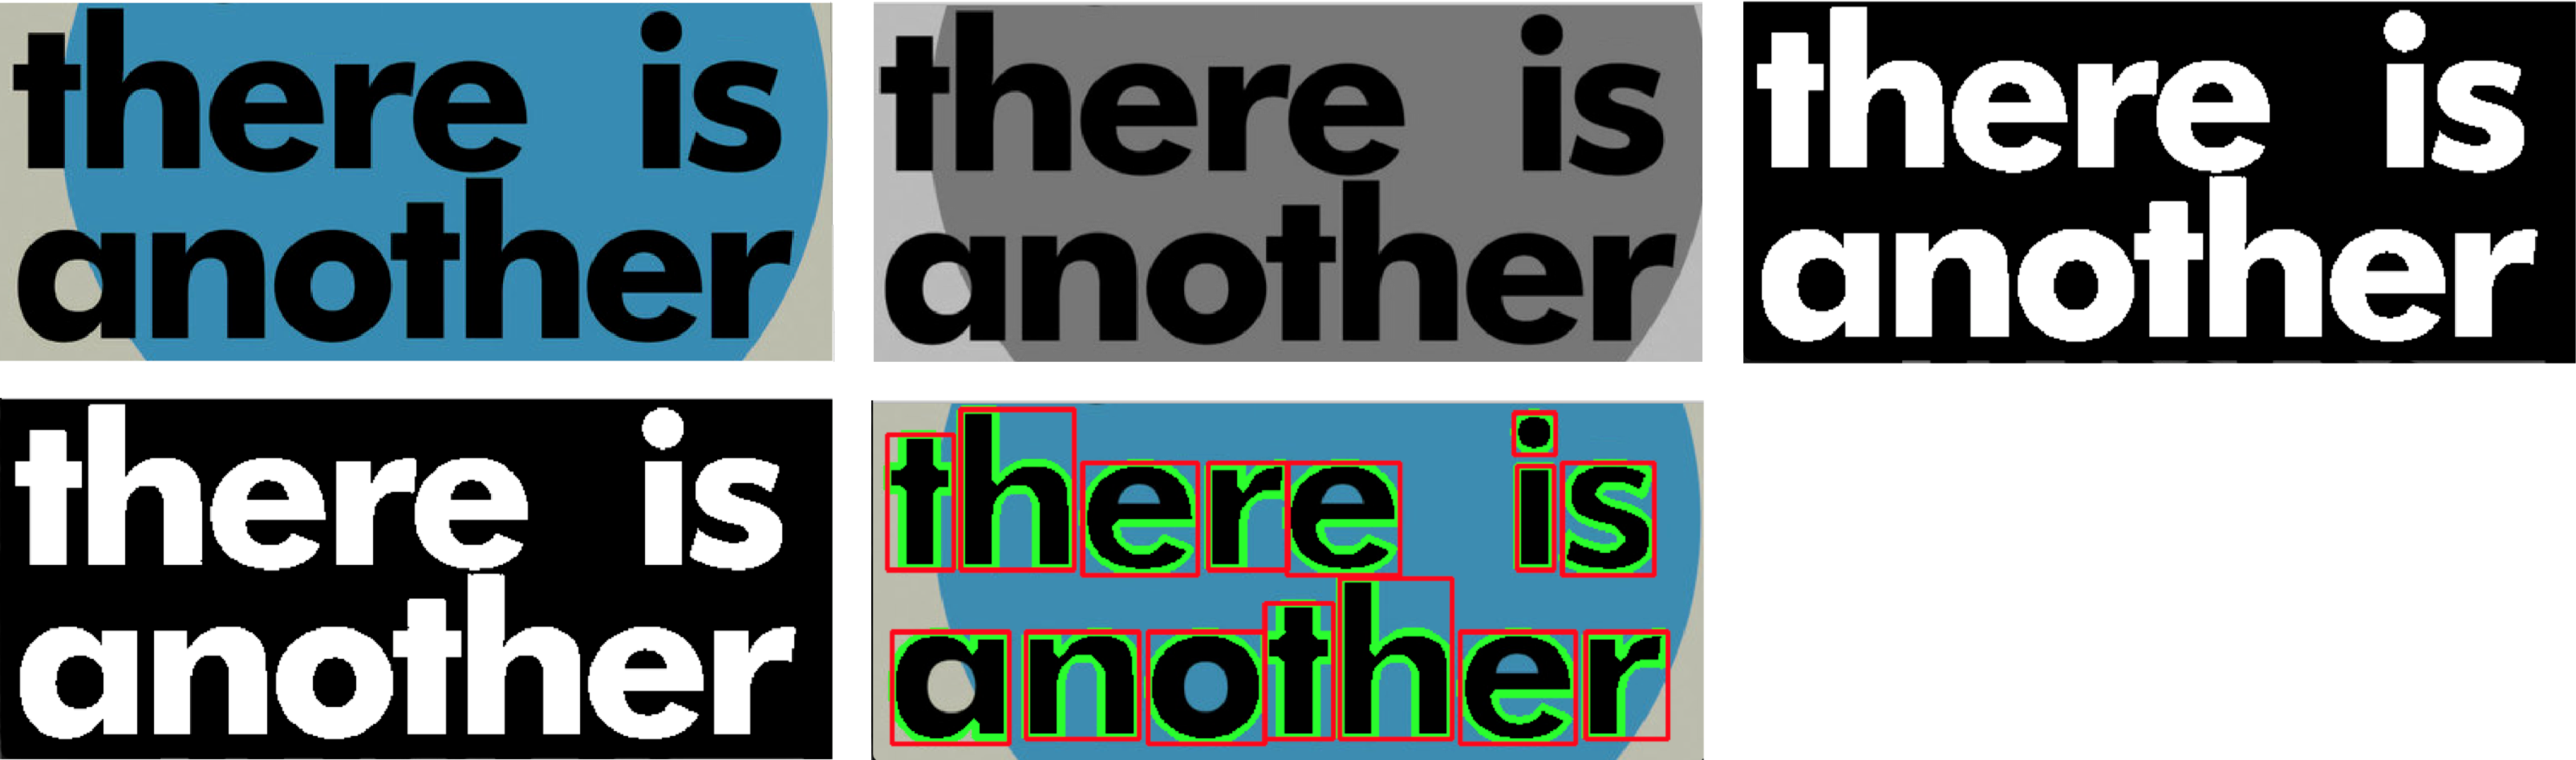
\includegraphics[width=0.9\linewidth]{figuras/imProcess2.pdf}
  \caption{Resultado por etapa do processo de reconhecimento de caracteres em imagens do banco de imagens. i)imagem original, ii)escala de cinza, iii)binarização inversa, iv)dilatação com \textit{kernel} em cruz e v)contornos e retângulos limitadores - \textbf{Fonte:} Autora}
  \label{fig:imProcess}
\end{figure}

Vale ressaltar que, por envolver um processo de binarização inversa no algoritmo, não foi possível efetuar a detecção de borda nas letras das imagens que, em escala de cinza, possuíam cor de fundo com tom mais escuro que aquele da letra. Portanto, se fez necessária uma correção na coloração de algumas imagens para melhor desempenho do algoritmo, processo realizado manualmente, no software \textit{Pré-Visualização} do sistema operacional \textit{Mac OS X} e também no software \textit{Adobe Lightroom}. Além disso, em algumas imagens, as letras em texto encontravam-se muito próximas uma à outra, o que gerou a demanda de uma limpeza de partes residuais de outras letras, após a formação das imagens de caracteres individuais.

O próximo método utilizado na seção principal do algoritmo é \texttt{imApaga}, responsável por excluir as imagens que possuem ambas dimensões inferiores a 45 pixels. O fluxograma descritivo pode ser visto na Figura \ref{fig:flowimApaga}.


\begin{figure}[H]
  \centering
  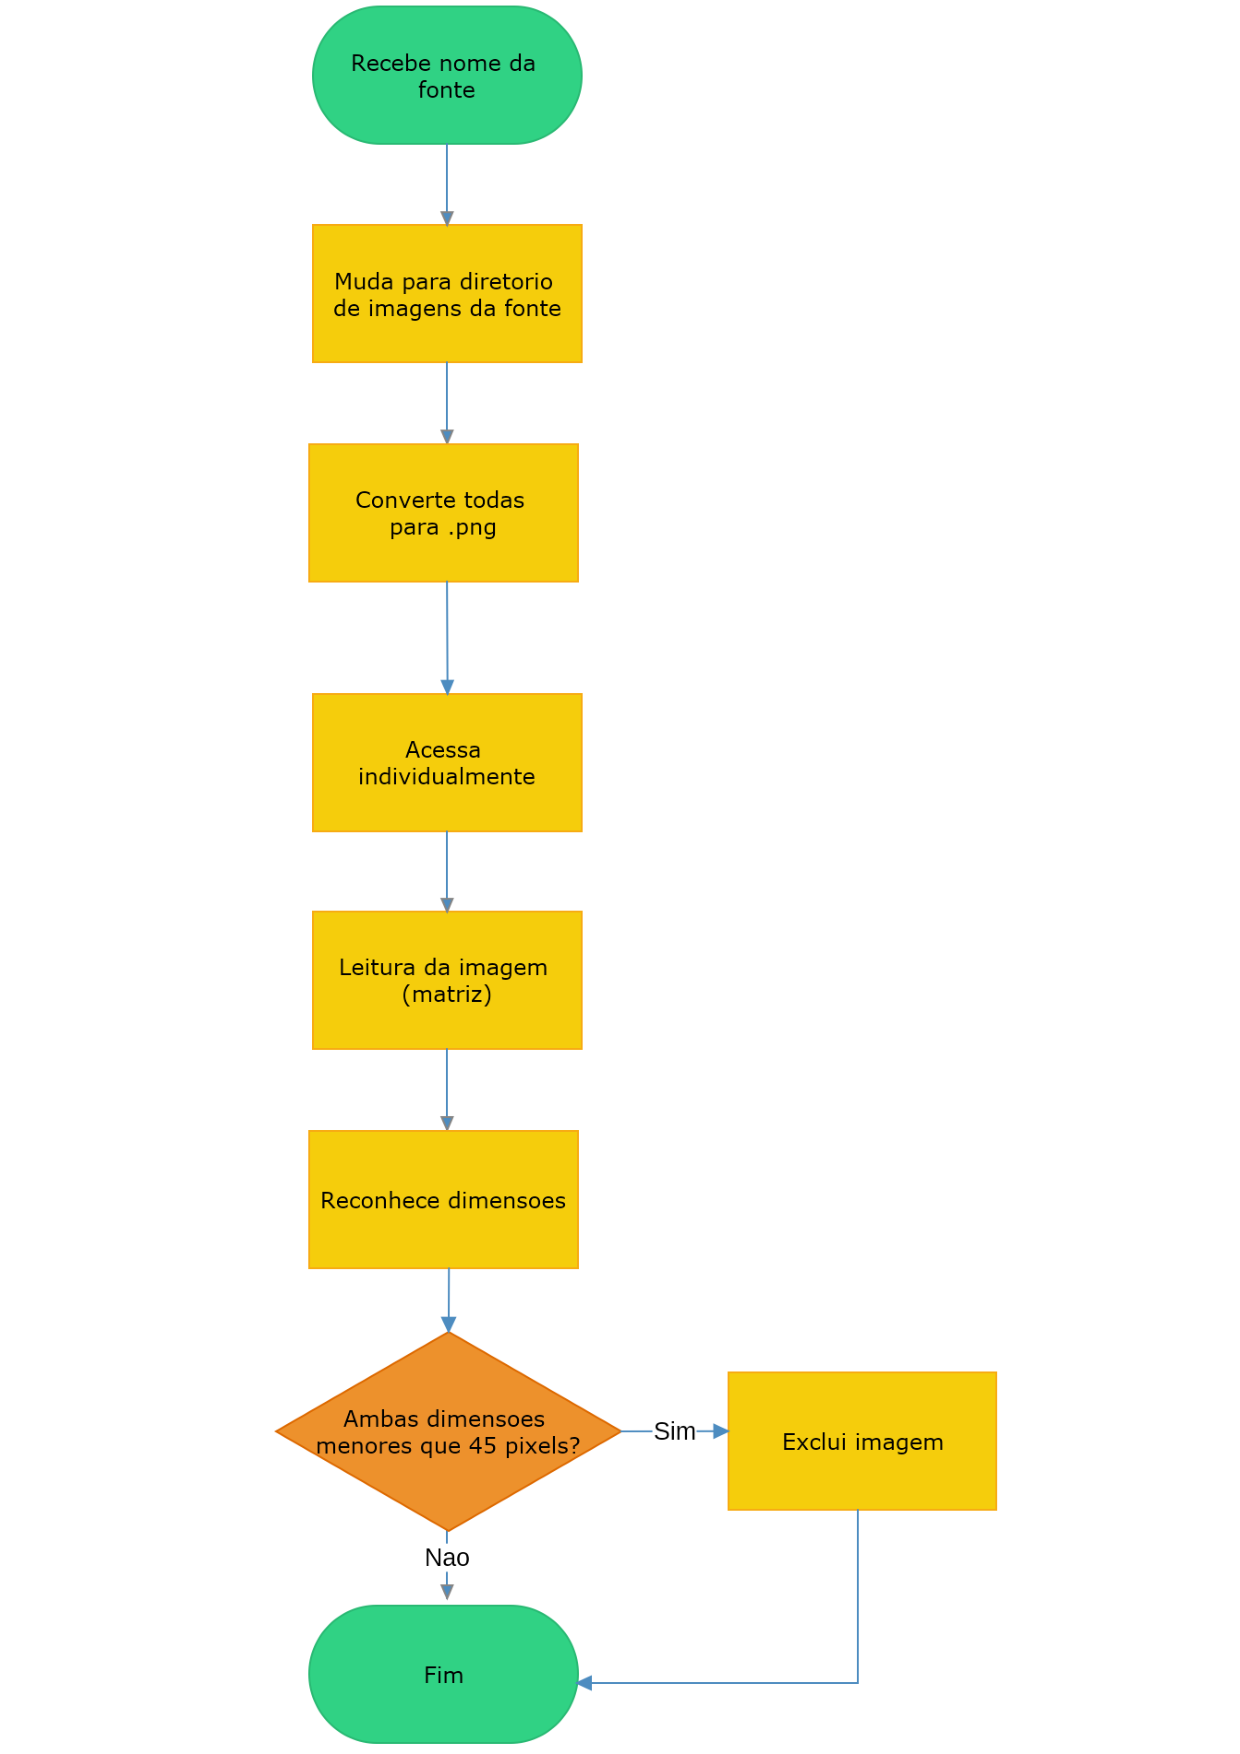
\includegraphics[width=0.8\linewidth]{figuras/imApaga.pdf}
  \caption{Fluxograma do método \texttt{imApaga} para excluir imagens com dimensões insatisfatórias - \textbf{Fonte:} Autora}
  \label{fig:flowimApaga}
\end{figure}

Assim como o método \texttt{imCrop}, recebe-se como parâmetro de entrada o nome da fonte em que se deseja operar e muda-se para o diretório do banco de imagens da fonte. Faz-se também a conversão de todas imagens para \textit{PNG}, que são depois acessadas individualmente e lidas, armazenando as intensidades dos pixels em uma matriz. Após isso, as dimensões da imagem são reconhecidas e avaliadas, caso as duas dimensões sejam menores que 45 pixels, a imagem é excluída, caso contrário, o programa passa para a próxima imagem, até finalizar todas presentes naquele diretório.

Por sua vez, o método \texttt{changeName} é utilizado para renomear as imagens presentes no diretório de acordo com a tipografia a que pertencem. A formatação padrão para o nome das imagens foi escolhida como: \textit{numero\_tipografia}. Por exemplo, o nome da sétima imagem presente no diretório da fonte Helvetica será "7\_helvetica". O caractere "\_" {} foi escolhido nesse caso para que a classe da imagem, a tipografia, seja de fácil identificação pelo algoritmo de treinamento do modelo classificador. O fluxograma desse método é apresentado na Figura \ref{fig:flowchangeName}.

Assim como os demais métodos dessa seção, começa-se recebendo o nome da fonte em qual se deseja operar e transfere-se para o diretório do banco de imagens dessa fonte. A biblioteca Python utilizada nesse método, a saber \textit{os}, ao renomear um arquivo, exclui o anterior que possui o mesmo nome. Portanto, para evitar que arquivos sejam excluídos erroneamente apenas por receberem nomes repetidos, primeiramente verifica-se se há o caractere "\_" {} no nome dos arquivos. Caso negativo, utiliza-se a nomenclatura padrão supracitada. Porém, caso positivo, nomeiam-se todos os arquivos com nomenclatura sem o caractere "\_" {} e, posteriormente, utiliza-se a nomenclatura padrão.

\begin{figure}[H]
  \centering
  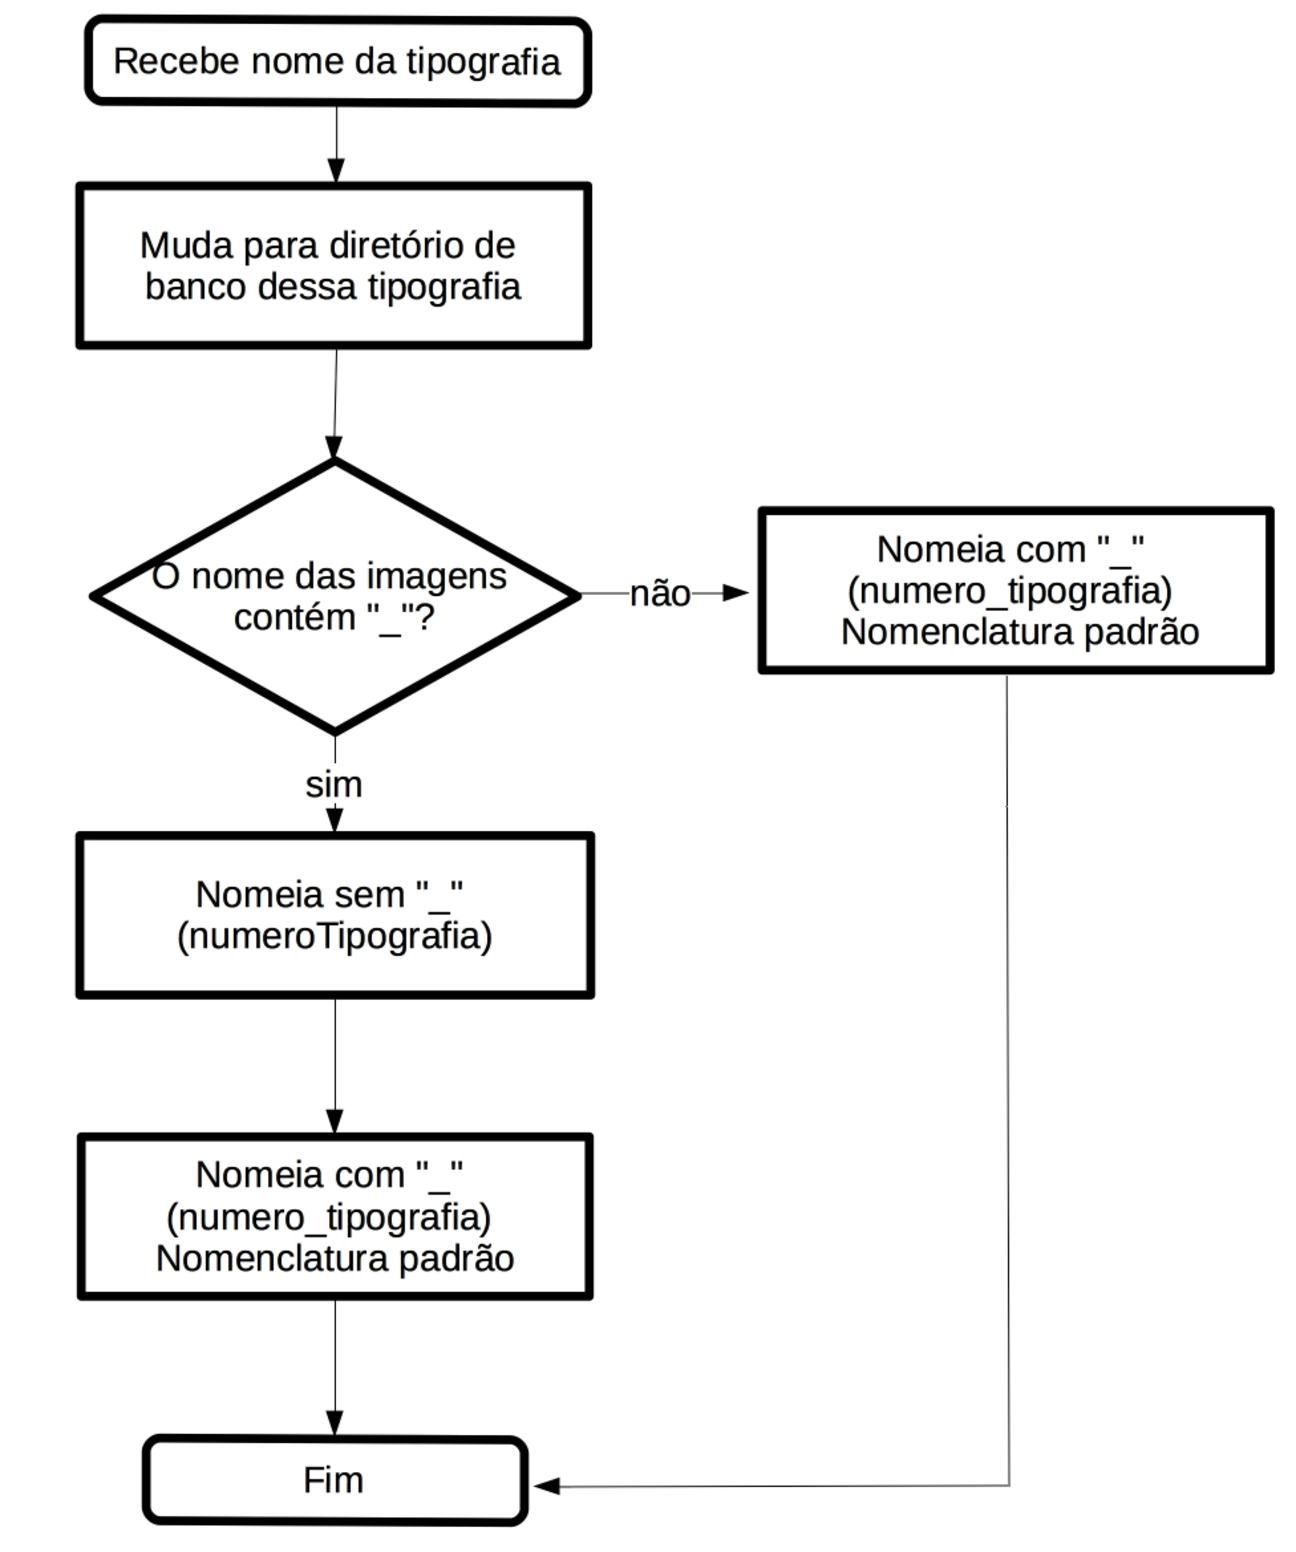
\includegraphics[width=0.6\linewidth]{figuras/changeName.pdf}
  \caption{Fluxograma do método \texttt{changeName} para renomear imagens de determinado diretório, preparando-as para o treinamento do modelo - \textbf{Fonte:} Autora}
  \label{fig:flowchangeName}
\end{figure}

O banco de imagens, em versão final, constitui-se de 6750 imagens no total, sendo 750 imagens por tipografia, com dimensão mínima de 45 pixels em altura ou largura. No entanto, inicialmente, para as primeiras quatro tipografias, o banco contava com 1895 imagens para cada uma delas. Porém, muitas imagens possuiam dimensão pequena, apresentando baixa resolução e ruídos, fato que comprometia o treinamento da máquina e, consequentemente, a acurácia do classificador. Sendo assim, decidiu-se reduzir o tamanho do banco de imagens, exluindo automaticamente aquelas que fossem menor do que a dimensão desejada. Além disso, em alguns casos, aprouve-se operar uma exclusão manual de imagens provenientes de erros de reconhecimento realizado pelo algoritmo ou que apresentavam baixa resolução, apesar de dimensão satisfatória.


%O processo de composição do banco de imagens para o treinamento do modelo a ser empregado na máquina foi a parte que mais demandou tempo em todo o processo de desenvolvimento do software. No entanto, em projetos nos quais a aprendizagem de máquina é utilizada essa etapa costuma ser descrita como demorada, como por exemplo (referência).


\section{Algoritmo para Treinamento do Modelo}

Essa seção destina-se à descrição do algoritmo implementado para treinamento do modelo da máquina e bem como de ferramentas utilizadas para seu desenvolvimento. O algoritmo é composto de três estágios, sendo que o resultado de um é o dado de entrada para o estágio subsequente:

\begin{enumerate}
\item Pré-processamento
\item Extração de atributos
\item Treinamento do modelo classificador e testes de predição
\end{enumerate}

O algoritmo foi também implementado em Python utilizando-se, como bibliotecas principais, as bibliotecas \textit{SciKit-learn}, \textit{SciKit-image}, \textit{NumPy} e, novamente, \textit{OpenCV}. Todas as bibliotecas citadas, exceto a \textit{OpenCV}, são derivadas de uma só coleção de bibliotecas, denominada \textit{SciPy}, que apresenta softwares de código livre para computação científica em Python. No entanto, as bibliotecas \textit{SciKit}, abreviação de \textit{SciPy Toolkits}, são pacotes complementares ao \textit{SciPy}, sendo desenvolvidas independentemente. O motivo de escolha dessas bibliotecas foi o mesmo apresentado anteriormente, são vastamente utilizadas na área de processamento de imagem e aprendizado de máquina \citeC{skimage2014}  \citeC{sklearn2011} \citeC{scipy2017} \citeC{numpy2017}.

\subsection{Estágio de pré-processamento}

Para essa etapa, a biblioteca \textit{OpenCV} foi a principal utilizada e implementado um processo similar ao método \texttt{imCrop} descrito na seção anterior. Todos os passos do pré-processamento encontram-se ilustrados na Figura \ref{fig:flowpreProc}.

\begin{figure}[H]
  \centering
  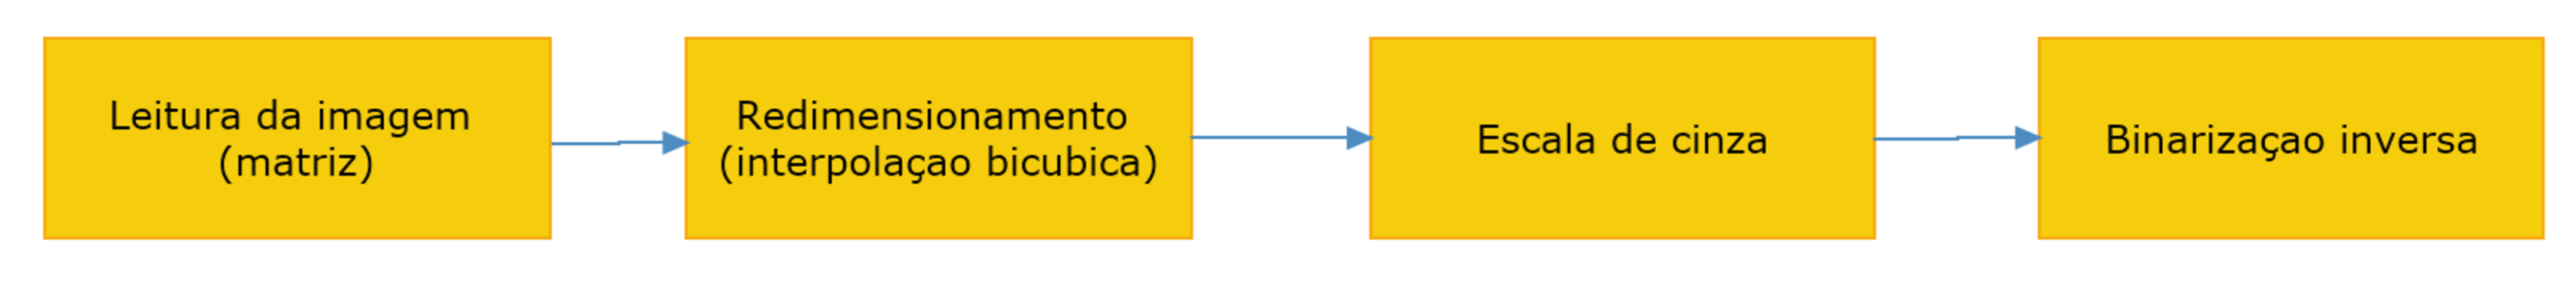
\includegraphics[width=1\linewidth]{figuras/preprocess.pdf}
  \caption{Etapas do estágio de pré-processamento do algoritmo de treinamento do modelo - \textbf{Fonte:} Autora}
  \label{fig:flowpreProc}
\end{figure}

Inicia-se pela leitura da imagem, transformando-a em matriz, seguido de seu redimensionamento por interpolação bicúbica para altura fixa de 126 pixels, garantindo, assim, uma melhor uniformidade das imagens para o processo de extração de atributos. O valor ótimo da nova dimensão foi encontrado por meio de iterações e testes de acurácia. Posteriormente, a imagem passa para escala de cinza e, por fim, é executada a binarização inversa da imagem. Todo esse processo é demonstrado como exemplo na Figura X.

%\begin{figure}[H]
%  \centering
%  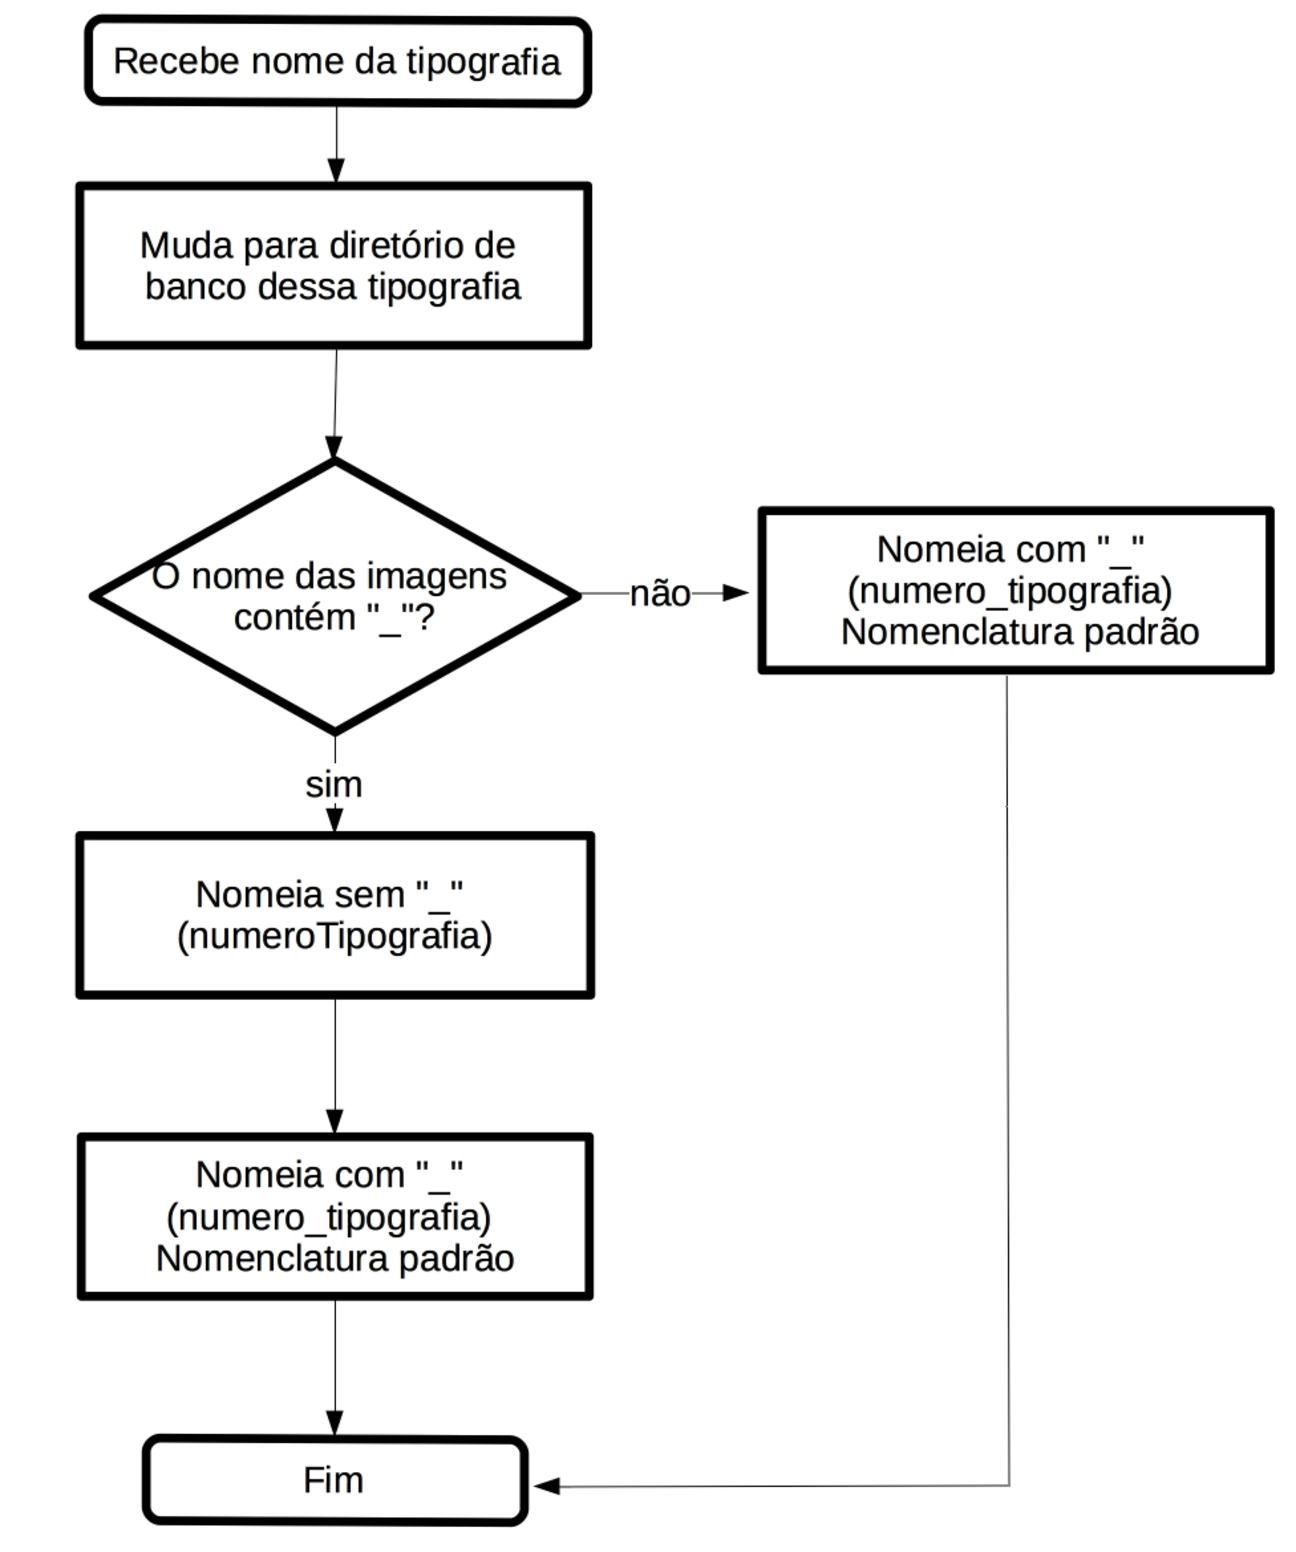
\includegraphics[width=0.6\linewidth]{figuras/changeName.pdf}
%  \caption{Fluxograma do método \texttt{changeName} para renomear imagens de determinado diretório, preparando-as para o treinamento do modelo - \textbf{Fonte:} Autora}
%  \label{fig:flowpreProc}
%\end{figure}

\subsection{Estágio de extração de atributos}

No estágio de extração de atributos, as bibliotecas usadas foram \textit{NumPy} e \textit{SciKit-image}. A biblioteca \textit{NumPy} é diretamente associada ao \textit{SciPy} e uma de suas vantagens principais é oferecer grande praticidade ao empregar matrizes, principalmente com uma vasta quantidade de elementos, por isso sendo bastante utilizada em aplicações com imagens, como no caso deste projeto.

Dessa mesma forma, a biblioteca \textit{SciKit-image} foi utilizada no algoritmo por ser uma biblioteca desenvolvida para processamento de imagem. Apenas um módulo da biblioteca, a saber \texttt{feature}, foi utilizado no algoritmo para fornecer a implementação da extração de atributos por meio do \textit{Local Binary Pattern} (LBP).

A seção de extração de atributos das imagens foi implementada como uma classe nomeada \texttt{LocalBinaryPattern}, em um módulo separado, e o modelo utilizado foi o LBP. Os parâmetros necessários para a sua aplicação na imagem, como explicado no capítulo 2, é o raio em relação ao pixel principal e a quantidade de pontos avaliados na circunferência de avaliação. Sendo assim, esses valores devem ser fornecidos ao se utilizar a classe na seção principal do algoritmo. Os valores adotados nesse caso foram um raio de 21 unidades e avaliação em 9 pontos, sendo encontrados por meio de um processo iterativo para determinar a combinação ótima.

Além disso, implementou-se um método, \texttt{describe}, para que o LBP de determinada imagem seja computado, todo o processo pode ser visto na Figura \ref{fig:flowLBP}. Logo, para haver a extração de atributos de uma imagem, esse método é chamado na seção principal do algoritmo, fornecido a ele o raio e o número de pontos desejados para o modelo e a imagem que será avaliada. Em seguida, o modelo em sua versão uniforme é aplicado na imagem, ou seja, sendo invariante à rotação e apresentando uma melhor quantização do espaço angular.

\begin{figure}[H]
  \centering
  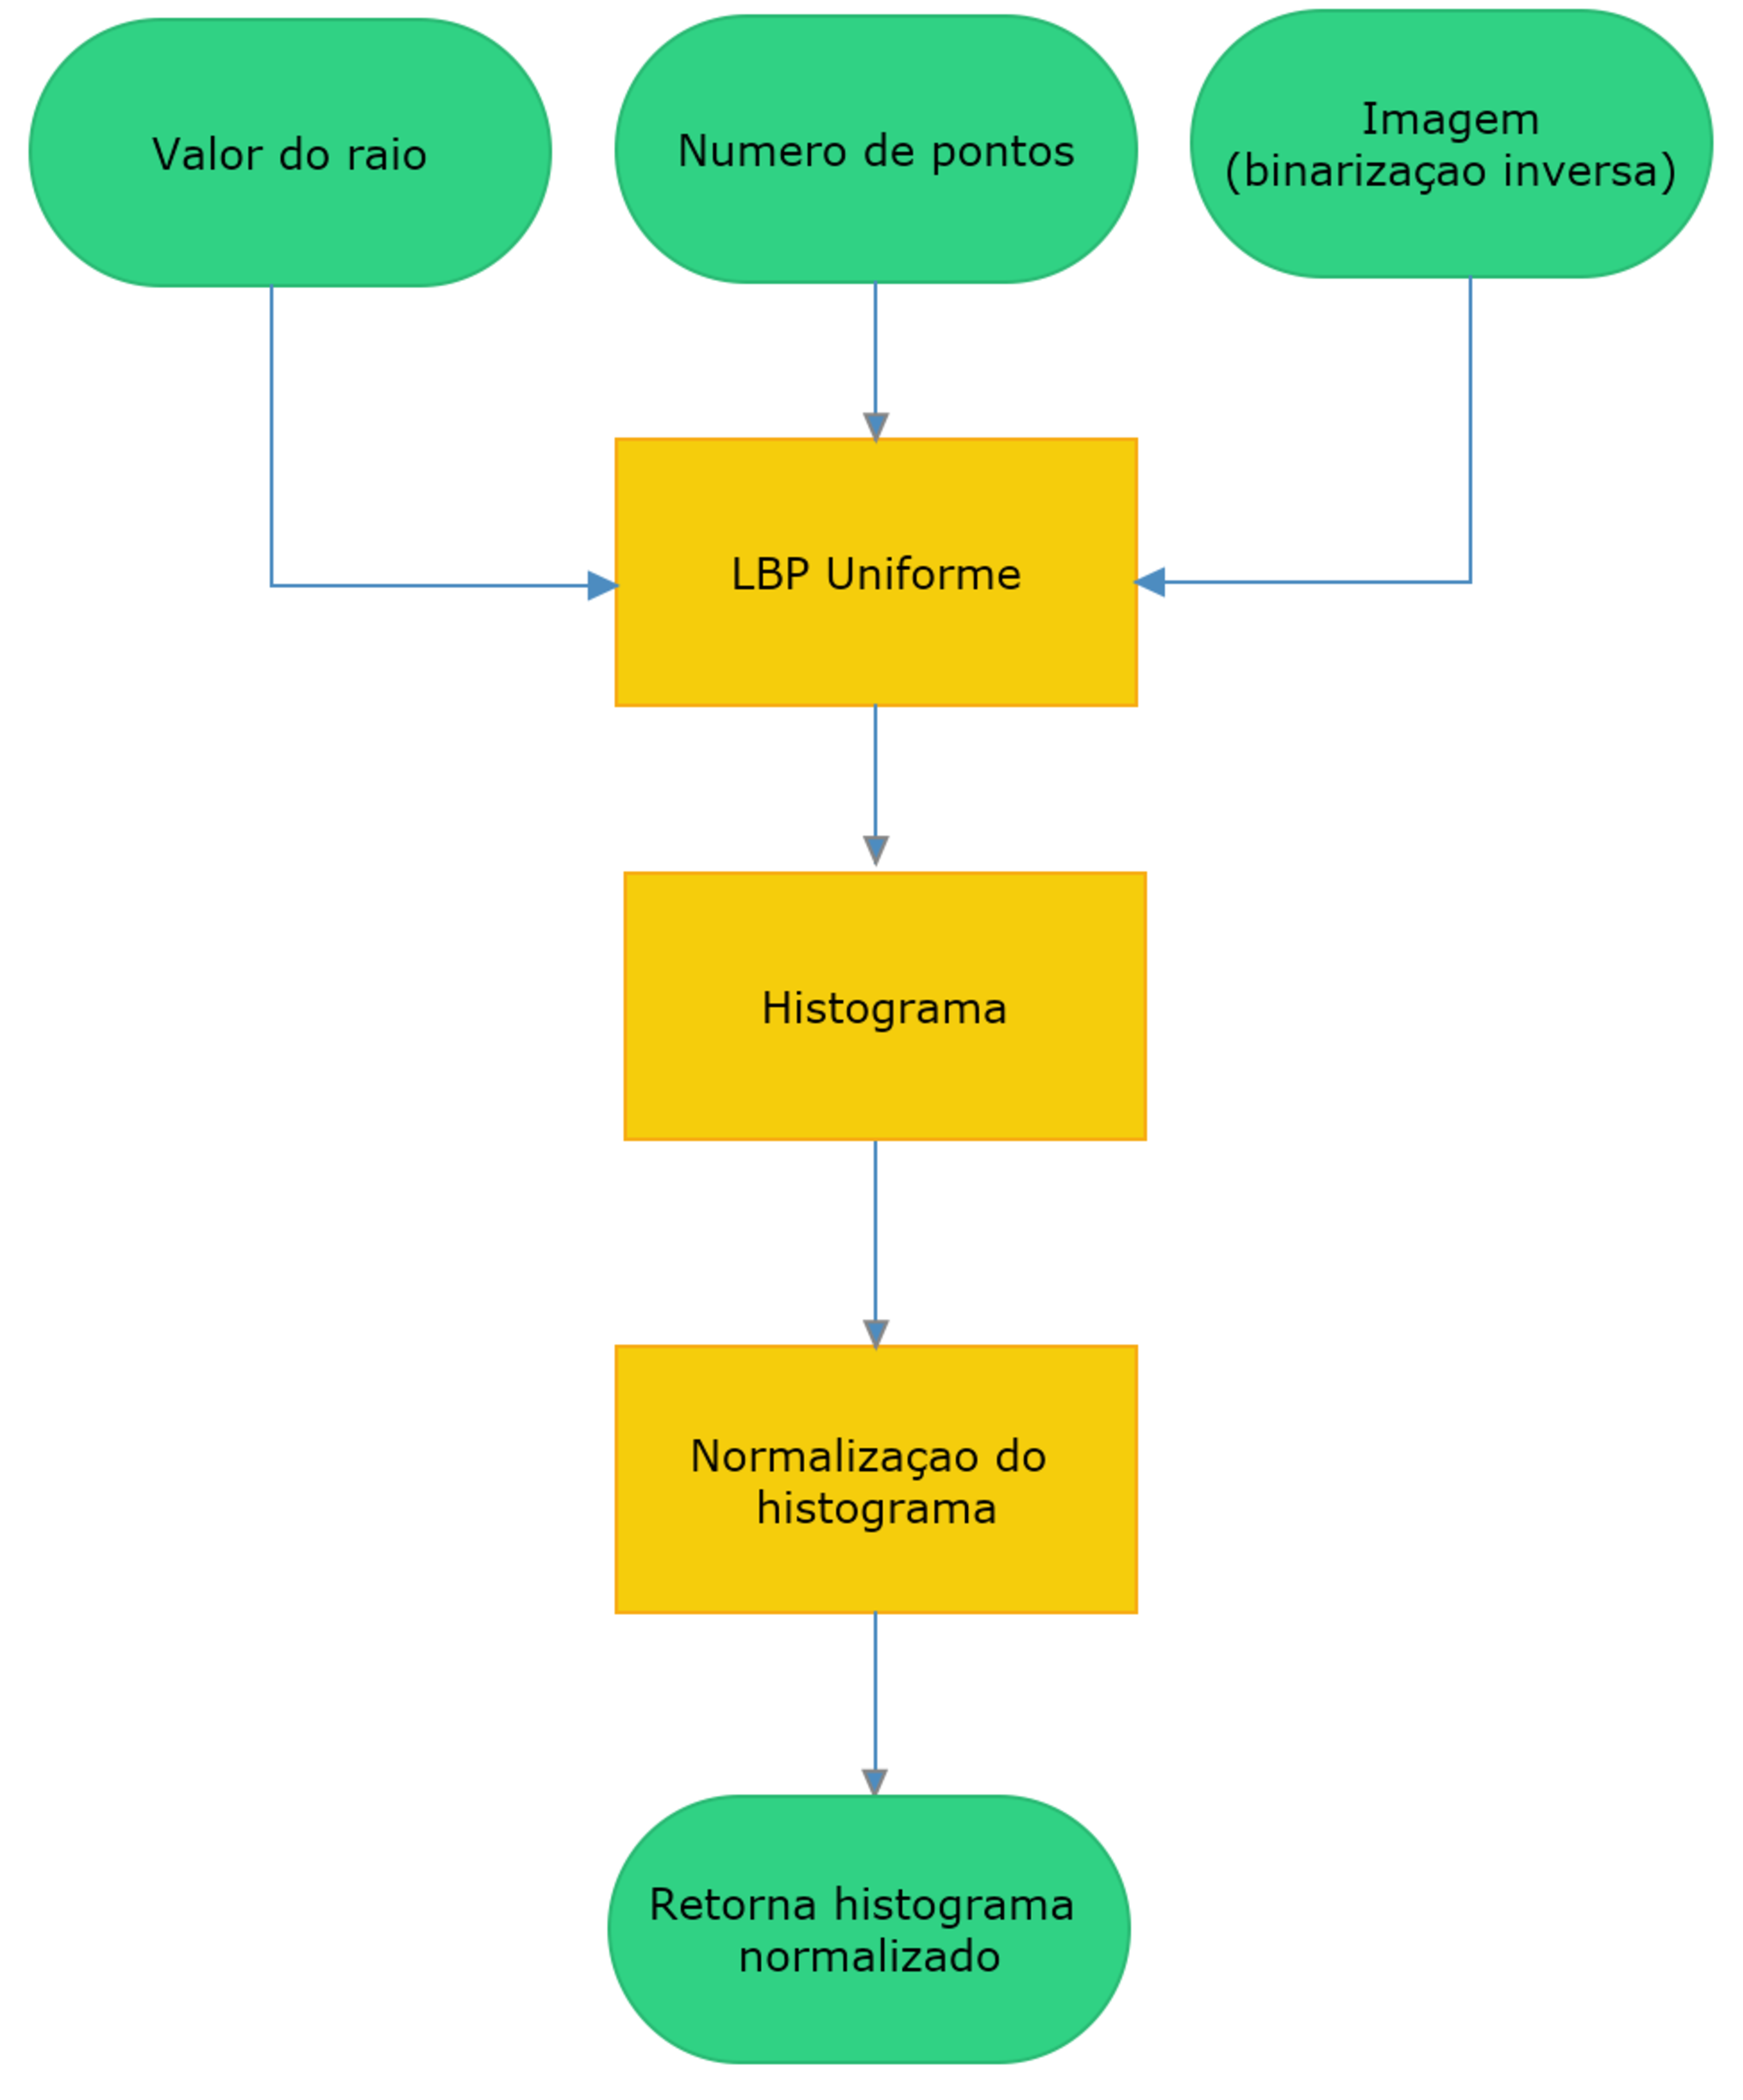
\includegraphics[width=0.75\linewidth]{figuras/lbp.pdf}
  \caption{Fluxograma do método \texttt{describe} para computar o LBP de uma imagem, retornando seu histograma normalizado - \textbf{Fonte:} Autora}
  \label{fig:flowLBP}
\end{figure}

Utilizando-se a biblioteca \textit{NumPy} para a estruturação e a manipulação dos vetores de atributos, o histograma da representação da imagem em LBP é então computado e normalizado, sendo retornado pelo método. O resultado de todo esse processo aplicado à amostras de imagens do banco de imagens é apresentado na Figura \ref{fig:nbinario} e, na Figura \ref{fig:nlbp}, é apresentam-se as imagens com binarização inversa que são as imagens de entrada no estágio.


\begin{figure}[H]
  \centering
  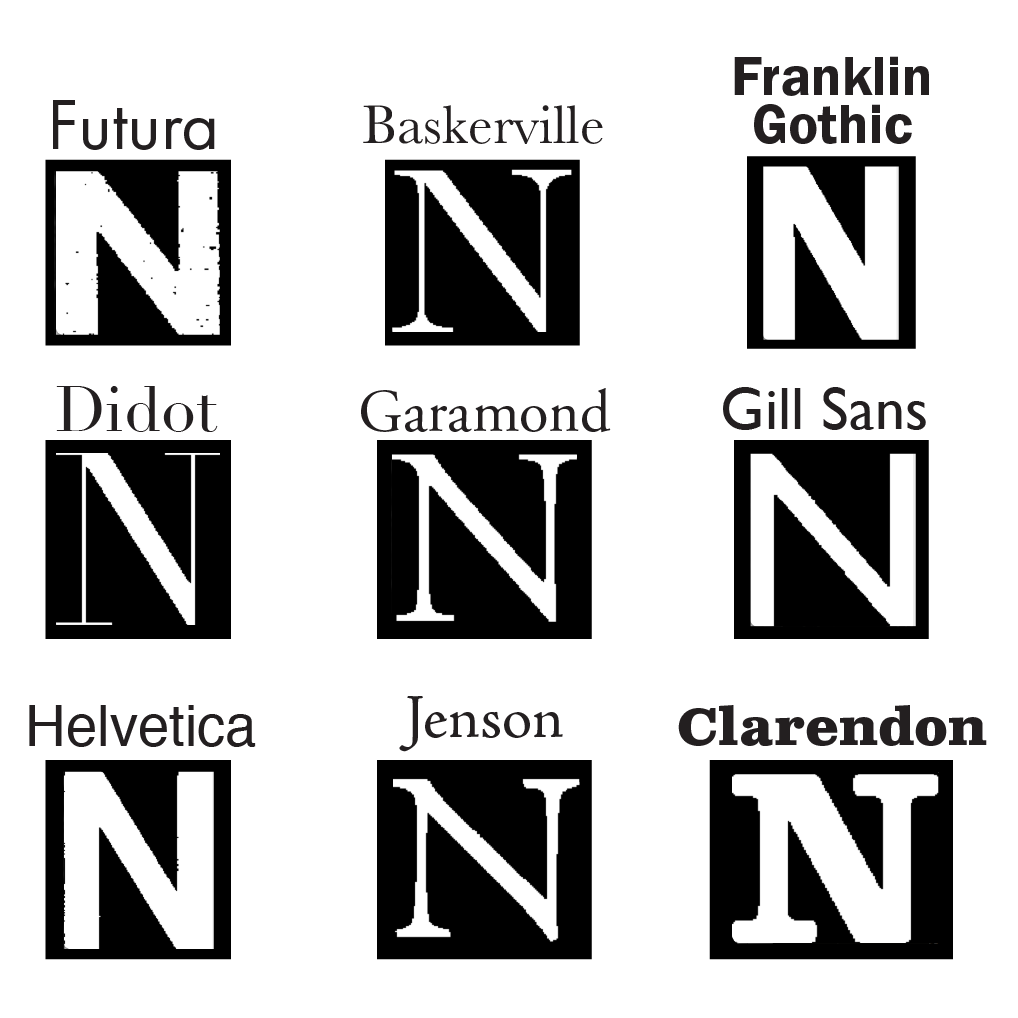
\includegraphics[width=0.6\linewidth]{figuras/nbinario.pdf}
  \caption{Amostras de imagens do banco de imagens após processo de binarização inversa. Imagens de entrada no estágio de extração de atributos  - \textbf{Fonte:} Autora}
  \label{fig:nbinario}
\end{figure}


\begin{figure}[H]
  \centering
  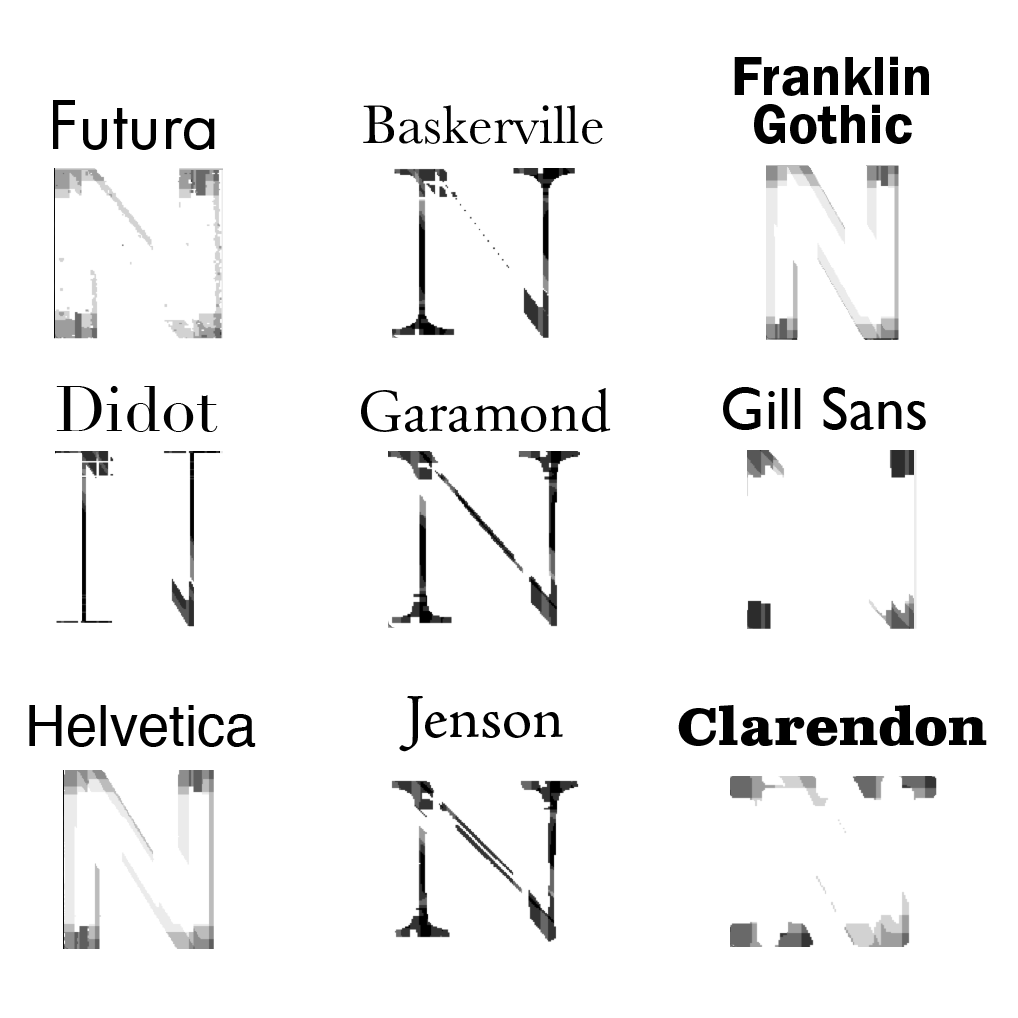
\includegraphics[width=0.6\linewidth]{figuras/nlbp.pdf}
  \caption{Amostras de imagens do banco de imagens após processo de extração de atributos, aplicação do LBP - \textbf{Fonte:} Autora}
  \label{fig:nlbp}
\end{figure}

%‘uniform’: improved rotation invariance with uniform patterns and finer quantization of the angular space which is gray scale and rotation invariant.

\subsection{Estágio de treinamento do modelo classificador e testes de predição}

Nesta etapa, a principal biblioteca utilizada foi a \textit{SciKit-learn}, que disponibiliza uma série de ferramentas para várias etapas pertinentes ao aprendizado de máquina. Os módulos utilizados, sendo eles \texttt{svm}, \texttt{ensemble}, \texttt{model\_selection}, \texttt{preprocessing}, oferecem os dois classificadores empregados, métricas para a escolha do modelo e outras ferramentas auxiliares, como a validação cruzada (\textit{Cross Validation}). Todo o processo do estágio de treinamento do classificador e testes de predição é descrito nos fluxogramas das Figuras \ref{fig:flowtreinamento1} e \ref{fig:flowtreinamento2}.

\begin{figure}[H]
  \centering
  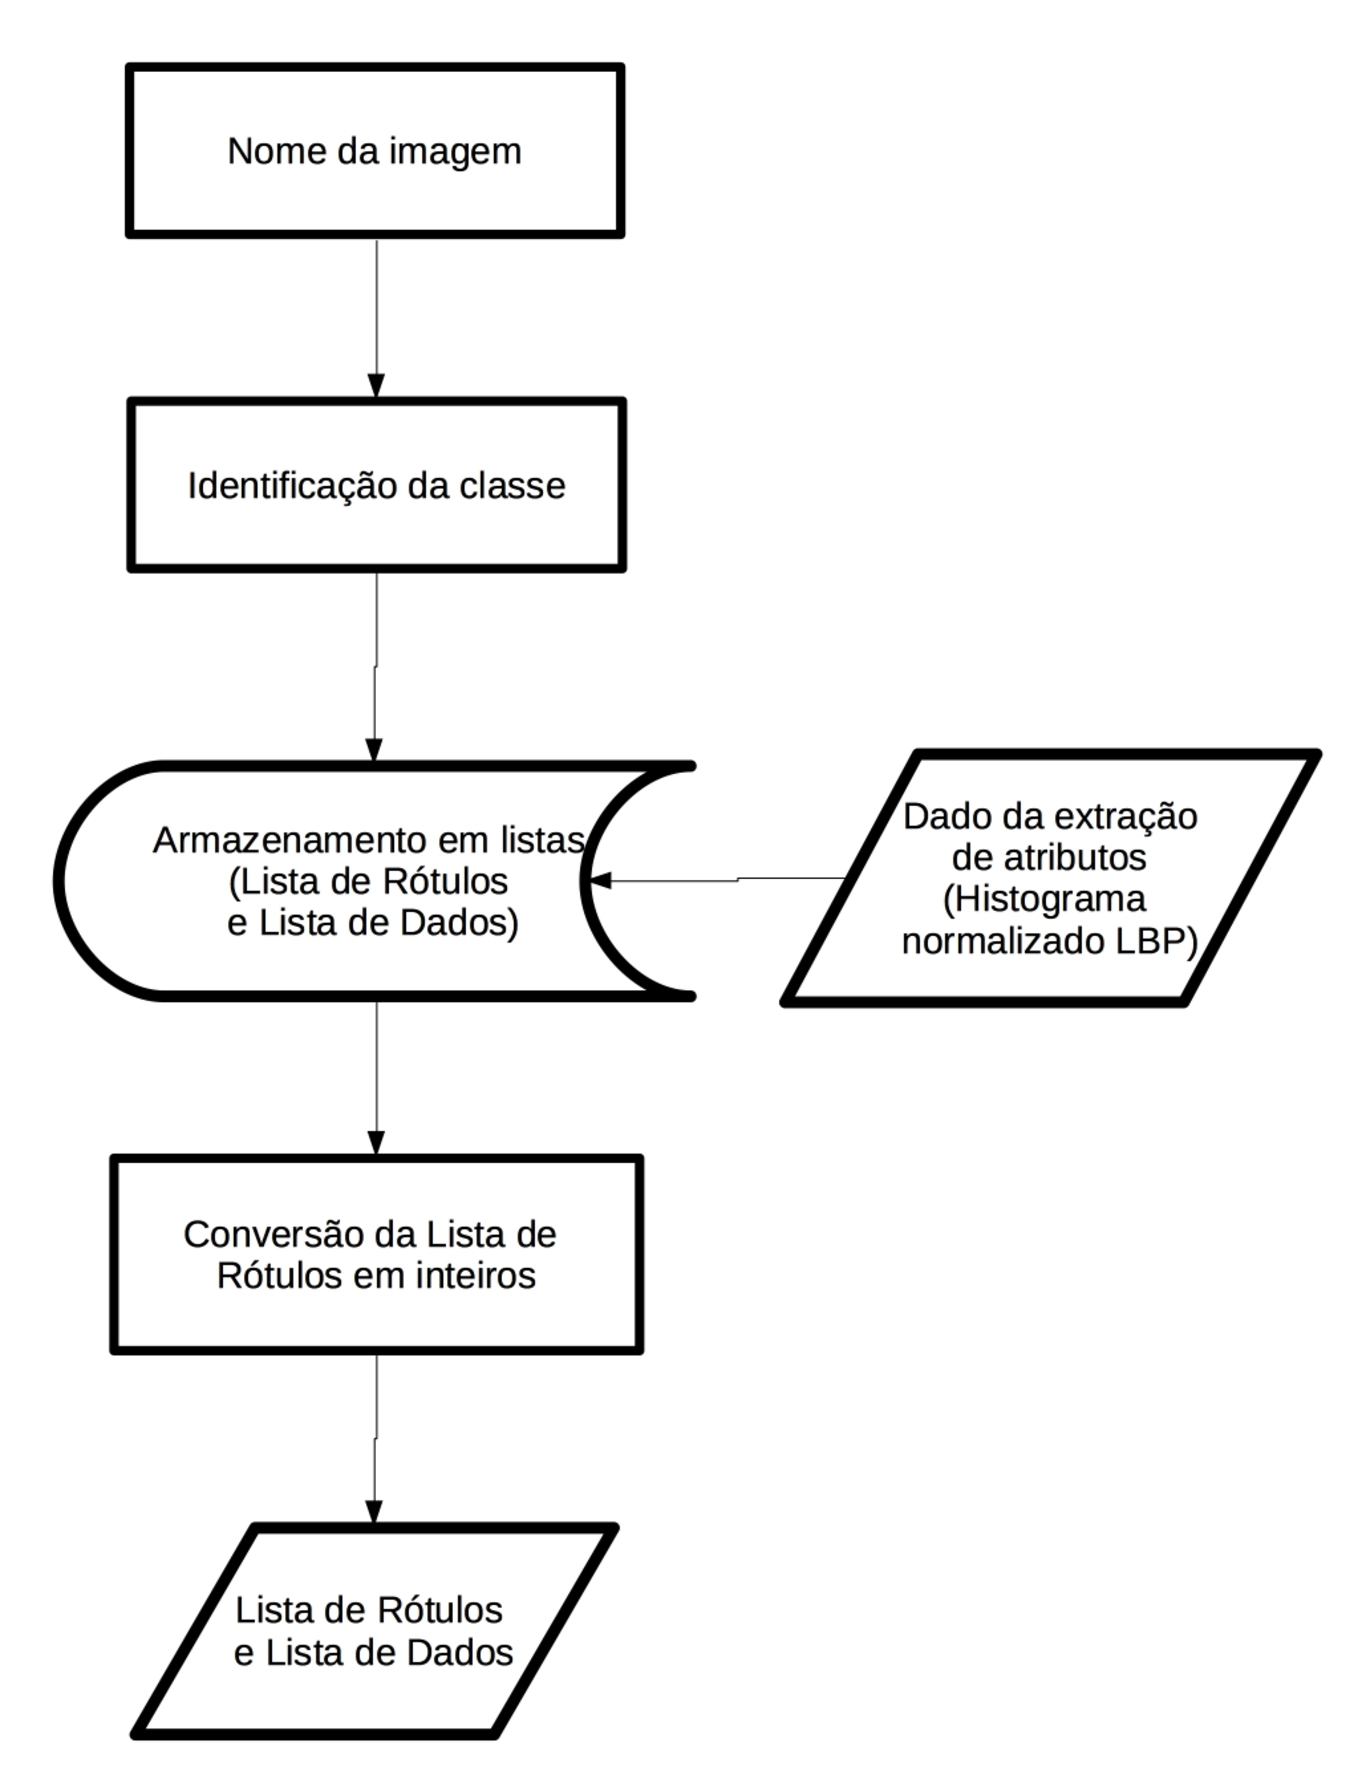
\includegraphics[width=0.6\linewidth]{figuras/treinamento1.pdf}
  \caption{Fluxograma da primeira parte do treinamento do modelo classificador, da extração da classe da imagem à formação das listas com os dados para treinamento - \textbf{Fonte:} Autora}
  \label{fig:flowtreinamento1}
\end{figure}

O estágio de treinamento do modelo classificador começa, então, com a extração da classe da imagem por meio do nome do arquivo. A imagem foi nomeada com o seguinte padrão: \textit{numero\_classe}, então o caractere "\_" {} é encontrado no nome do arquivo e a palavra contida após ele é reservada como a classe da imagem. O histograma do LBP daquela imagem é também reservado, sendo relacionado à classe por partilharem de mesma posição na lista de armazenamento de classes e de dados (histogramas). Esse processo é feito imagem a imagem. Para tornar o processamento mais eficiente, a lista de classes obtidas a partir das imagens é convertida para uma lista de inteiros, na qual cada número representa uma classe.

Nesta etapa, dois modelos foram usados para a classificação das imagens. Primeiramente, utilizou-se o classificador Máquina de Vetor de Suporte (SVM, em inglês \textit{Support Vector Machine}) em sua versão linear. Porém, por apresentar um resultado insatisfatório, fato explicitado no próximo capítulo, um novo modelo de classificador foi adotado, \textit{Random Forest Classifier} (RF).

Para o caso do SVM, foram fornecidos ao modelo alguns parâmetros para sua estruturação, nesse caso, o parâmetro de penalidade \textit{C} do termo erro na classificação, adotado como 100, e o estado randômico (\textit{random state}) para o embaralhamento das imagens, adotado o valor unitário. Para o caso do \textit{Random Forest Classifier}, os parâmetros fornecidos são o número de árvores de decisão, utilizou-se 82, e o número de tarefas que irão ser realizadas em paralelo, ajustou-se para a execução de número máximo de tarefas em paralelo.

Após isso, passa-se para o ajuste dos parâmetros da validação cruzada a ser utilizada, no caso \textit{Stratified K Fold}. Utilizando essa implementação de validação cruzada, uma variação do modelo \textit{K Fold},  no processo de divisão em subconjuntos (pastas), a porcentagem de amostras de cada classe é mantida de acordo com o conjunto original das imagens. Os parâmetros referentes à validação cruzada utilizada são o número de subconjuntos em que as imagens serão divididas, adotado como sete neste projeto, a opção de embaralhamento e, como no classificador, o estado randômico para o embaralhamento, no qual foi usado valor unitário.

Em sequência, o classificador é aplicado no conjunto de imagens, o processo é todo operado utilizando a validação cruzada previamente ajustada, ou seja, o treinamento é feito e também o teste da predição. Baseada em todas as iterações da validação cruzada, a acurácia da classificação é calculada, sua média e desvio padrão.

\begin{figure}[H]
 \centering
  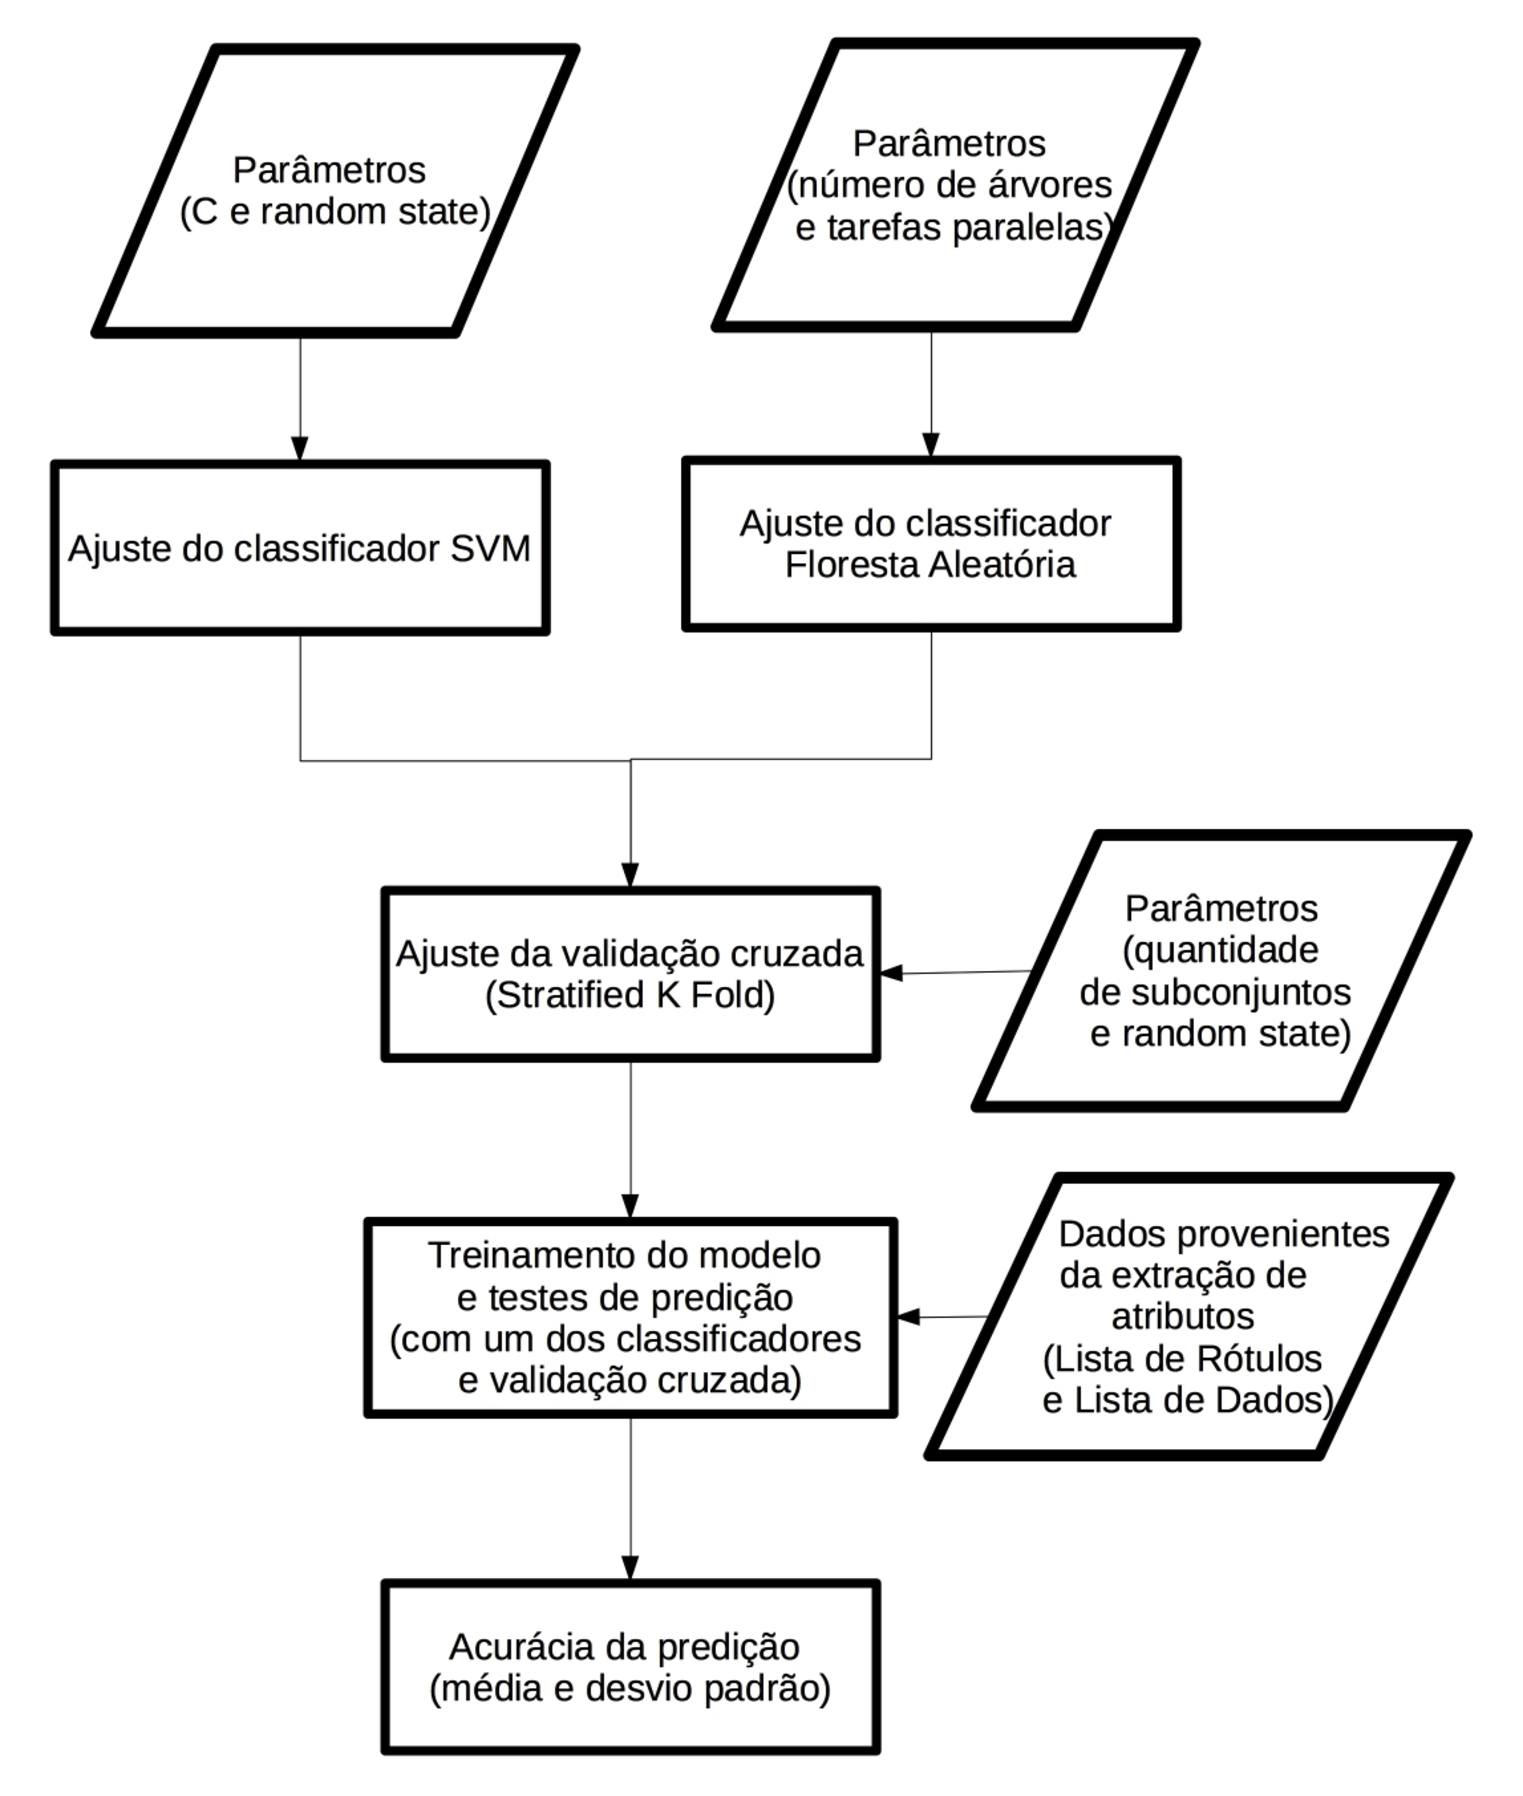
\includegraphics[width=0.7\linewidth]{figuras/treinamento2.pdf}
  \caption{Fluxograma da segunda parte do treinamento do modelo classificador, do ajuste dos modelos classificadores ao resultado de acurácia das predições - \textbf{Fonte:} Autora}
  \label{fig:flowtreinamento2}
\end{figure}

Todo o processo descrito nessa seção foi realizado em várias iterações, com a variação de muitos parâmetros que compõem os modelos para que os valores ótimos fossem encontrados. Todos seus resultados serão apresentados no capítulo seguinte.


%metodologia de outro artigo
%The methodology applied in our processing im- age algorithm was based on to estimate features not over full image, instead of this, feature estima- tionwasdoneoverregionsofimagescalled‘‘sub- image’’.Theestimatedattributearraysofeach sub-image were the reference database to recognize thetypeofeachfont(100windowsaretakenran- domlyovereachfulltext) \citeC{aviles2005}


%A \textit{NumPy} foi ainda utilizada no desenvolvimento das duas bibliotecas \textit{SciKit} aqui empregadas. No escopo do algoritmo desenvolvido para o treinamento do modelo de classificação das tipografias, a \textit{NumPy} foi empregue, principalmente, na etapa de pré-processamento e extração de atributos das imagens.



